\begin{figure}[htbp!]
	\begin{center}
	
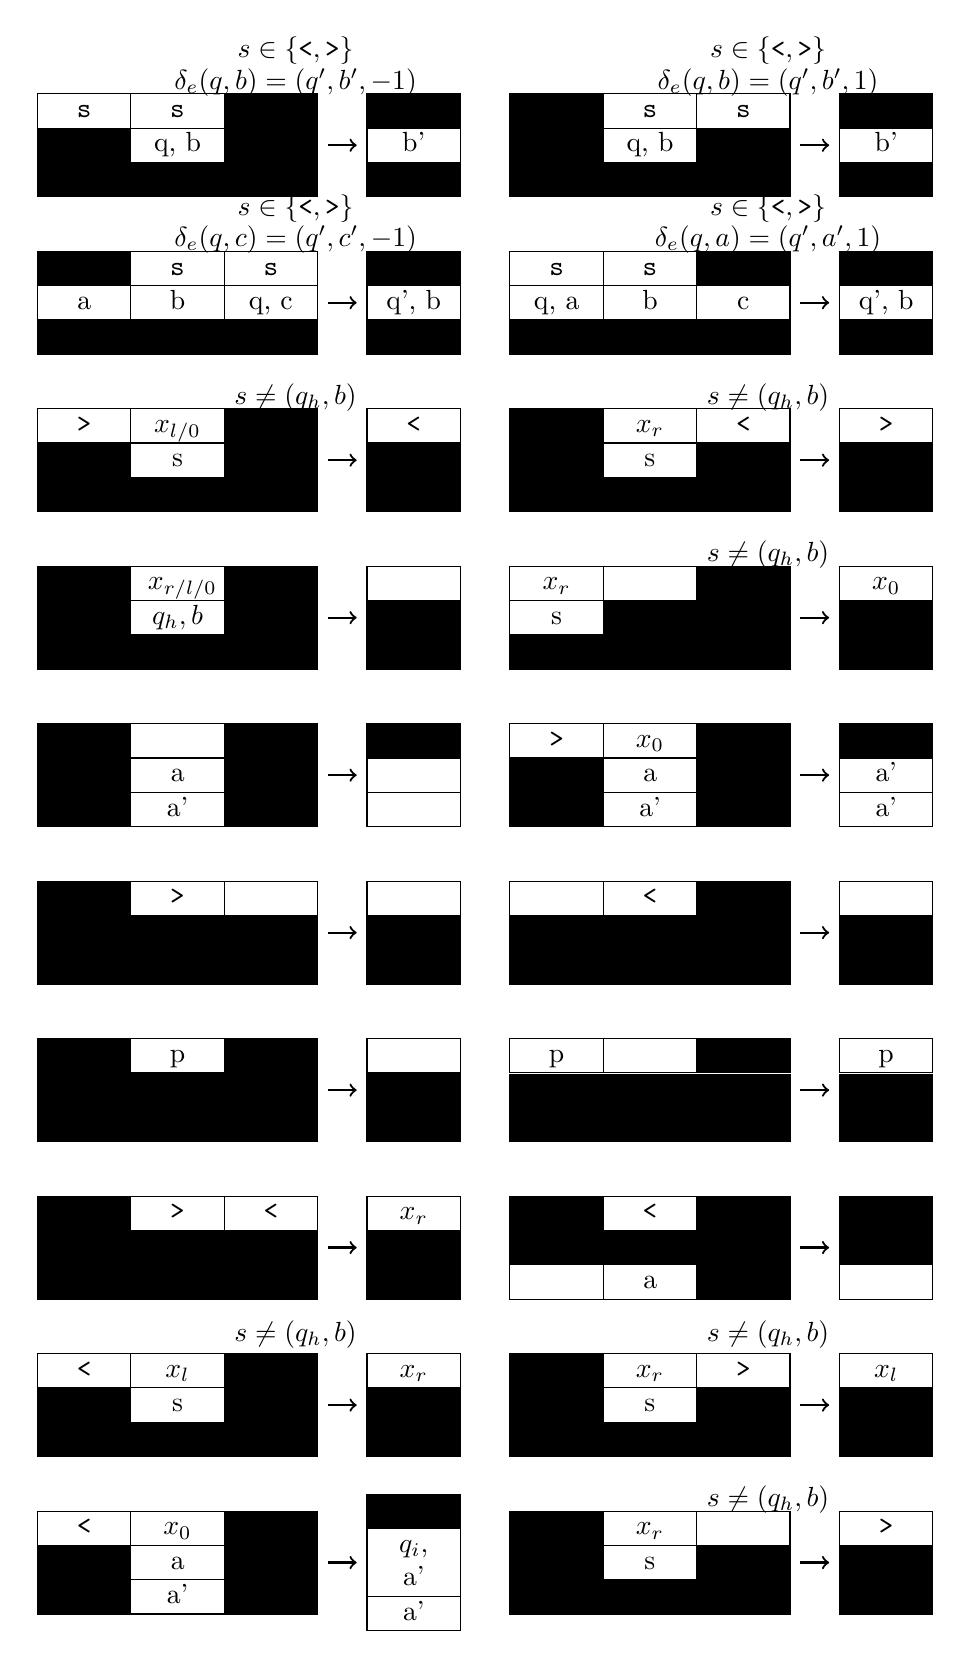
\begin{tikzpicture}

    % règle 1
    \node (tab1) at (0,0) {
        \begin{tabular}{| >{\centering\arraybackslash}m{0.75cm}| >{\centering\arraybackslash}m{0.75cm}| >{\centering\arraybackslash}m{0.75cm}|}
        \hline
        \texttt{s} & \texttt{s} & \cellcolor{black}~ \\
        \hline
	\cellcolor{black}~ & q, b & \cellcolor{black} \\
        \hline
        \cellcolor{black} & \cellcolor{black} & \cellcolor{black} \\
        \hline
        \end{tabular}
    };

    \node (tab2) at (3, 0){
        \begin{tabular}{| >{\centering\arraybackslash}m{0.75cm}| >{\centering\arraybackslash}m{0.75cm}| >{\centering\arraybackslash}m{0.75cm}|}
        \hline
	\cellcolor{black}\\
	\hline
	b'\\
        \hline
          \cellcolor{black} \\
        \hline
        \end{tabular}
    };

    \draw[->, thick] (tab1) -- (tab2);
    \node at (1.5, 0.8) {$\delta_e(q, b) = (q', b',  -1)$};
    \node at (1.5, 1.2) {$s \in \{\texttt{<}, \texttt{>}\}$};
    
    % règle 2
    \node (tab3) at (6,0) {
        \begin{tabular}{| >{\centering\arraybackslash}m{0.75cm}| >{\centering\arraybackslash}m{0.75cm}| >{\centering\arraybackslash}m{0.75cm}|}
        \hline
        \cellcolor{black} & \texttt{s} & \texttt{s}\\
        \hline
	\cellcolor{black} & q, b & \cellcolor{black} \\
        \hline
        \cellcolor{black} & \cellcolor{black} & \cellcolor{black} \\
        \hline
        \end{tabular}
    };

    \node (tab4) at (9,0) {
        \begin{tabular}{| >{\centering\arraybackslash}m{0.75cm}| >{\centering\arraybackslash}m{0.75cm}| >{\centering\arraybackslash}m{0.75cm}|}
        \hline
	\cellcolor{black} \\
        \hline
         b'  \\
        \hline
        \cellcolor{black} \\
        \hline
        \end{tabular}
    };
    \draw[->, thick] (tab3) -- (tab4);
    \node at (7.5, 0.8) {$\delta_e(q, b) = (q', b', 1)$};
     \node at (7.5, 1.2) {$s \in \{\texttt{<}, \texttt{>}\}$};

    % règle 3
    \node (tab5) at (0,-2) {
        \begin{tabular}{| >{\centering\arraybackslash}m{0.75cm}| >{\centering\arraybackslash}m{0.75cm}| >{\centering\arraybackslash}m{0.75cm}|}
        \hline
        \cellcolor{black} & \texttt{s} & \texttt{s} \\
        \hline
	a & b & q, c \\
        \hline
        \cellcolor{black} & \cellcolor{black} & \cellcolor{black} \\
        \hline
        \end{tabular}
    };

    \node (tab6) at (3,-2) {
        \begin{tabular}{| >{\centering\arraybackslash}m{0.75cm}| >{\centering\arraybackslash}m{0.75cm}| >{\centering\arraybackslash}m{0.75cm}|}
        \hline
	\cellcolor{black} \\
        \hline
        q', b \\
        \hline
          \cellcolor{black} \\
        \hline
        \end{tabular}
    };
    \draw[->, thick] (tab5) -- (tab6);
    \node at (1.5, -1.2) {$\delta_e(q, c) = (q', c', -1)$};
     \node at (1.5, -0.8) {$s \in \{\texttt{<}, \texttt{>}\}$};
    
    % règle 4
    \node (tab7) at (6,-2) {
        \begin{tabular}{| >{\centering\arraybackslash}m{0.75cm}| >{\centering\arraybackslash}m{0.75cm}| >{\centering\arraybackslash}m{0.75cm}|}
        \hline
        \texttt{s} & \texttt{s} & \cellcolor{black} \\
        \hline
	q, a & b & c \\
        \hline
        \cellcolor{black} & \cellcolor{black} & \cellcolor{black} \\
        \hline
        \end{tabular}
    };

    \node (tab8) at (9, -2){
        \begin{tabular}{| >{\centering\arraybackslash}m{0.75cm}| >{\centering\arraybackslash}m{0.75cm}| >{\centering\arraybackslash}m{0.75cm}|}
        \hline
        \cellcolor{black} \\
        \hline
	q', b \\
        \hline
          \cellcolor{black} \\
        \hline
        \end{tabular}
    };

    \draw[->, thick] (tab7) -- (tab8);
    \node at (7.5, -1.2) {$\delta_e(q, a) = (q', a', 1)$};
     \node at (7.5, -0.8) {$s \in \{\texttt{<}, \texttt{>}\}$};
    
    % règle 5
    \node (tab9) at (0,-4) {
        \begin{tabular}{| >{\centering\arraybackslash}m{0.75cm}| >{\centering\arraybackslash}m{0.75cm}| >{\centering\arraybackslash}m{0.75cm}|}
        \hline
        \texttt{>} & $x_{l/0}$ & \cellcolor{black}\\
        \hline
	\cellcolor{black} & s & \cellcolor{black} \\
        \hline
        \cellcolor{black} & \cellcolor{black} & \cellcolor{black} \\
        \hline
        \end{tabular}
    };

    \node (tab10) at (3,-4) {
        \begin{tabular}{| >{\centering\arraybackslash}m{0.75cm}| >{\centering\arraybackslash}m{0.75cm}| >{\centering\arraybackslash}m{0.75cm}|}
        \hline
	\texttt{<} \\
        \hline
        \cellcolor{black} \\
        \hline
          \cellcolor{black} \\
        \hline
        \end{tabular}
    };
    \draw[->, thick] (tab9) -- (tab10);
    \node at (1.5, -3.2) {$s \neq (q_h, b)$};
    
    % règle 6
    \node (tab11) at (6,-4) {
        \begin{tabular}{| >{\centering\arraybackslash}m{0.75cm}| >{\centering\arraybackslash}m{0.75cm}| >{\centering\arraybackslash}m{0.75cm}|}
        \hline
        \cellcolor{black} & $x_r$ & \texttt{<} \\
        \hline
	\cellcolor{black}  & s & \cellcolor{black} \\
        \hline
        \cellcolor{black} & \cellcolor{black} & \cellcolor{black} \\
        \hline
        \end{tabular}
    };

    \node (tab12) at (9, -4){
        \begin{tabular}{| >{\centering\arraybackslash}m{0.75cm}| >{\centering\arraybackslash}m{0.75cm}| >{\centering\arraybackslash}m{0.75cm}|}
        \hline
        \texttt{>} \\
        \hline
	\cellcolor{black}  \\
        \hline
          \cellcolor{black} \\
        \hline
        \end{tabular}
    };

    \draw[->, thick] (tab11) -- (tab12);
    \node at (7.5, -3.2) {$s \neq (q_h, b)$};
    
    % règle 7
    \node (tab13) at (0,-6) {
        \begin{tabular}{| >{\centering\arraybackslash}m{0.75cm}| >{\centering\arraybackslash}m{0.75cm}| >{\centering\arraybackslash}m{0.75cm}|}
        \hline
        \cellcolor{black} & $x_{r/l/0}$ & \cellcolor{black}\\
        \hline
	\cellcolor{black} & $q_h, b$ & \cellcolor{black} \\
        \hline
        \cellcolor{black} & \cellcolor{black} & \cellcolor{black} \\
        \hline
        \end{tabular}
    };

    \node (tab14) at (3,-6) {
        \begin{tabular}{| >{\centering\arraybackslash}m{0.75cm}| >{\centering\arraybackslash}m{0.75cm}| >{\centering\arraybackslash}m{0.75cm}|}
        \hline
	 \\
        \hline
        \cellcolor{black} \\
        \hline
          \cellcolor{black} \\
        \hline
        \end{tabular}
    };
    \draw[->, thick] (tab13) -- (tab14);
    %\node at (1.5, -5.2) {$\delta_e(q, c) = (q', c', -1)$};
    
    % règle 8
    \node (tab15) at (6,-6) {
        \begin{tabular}{| >{\centering\arraybackslash}m{0.75cm}| >{\centering\arraybackslash}m{0.75cm}| >{\centering\arraybackslash}m{0.75cm}|}
        \hline
        $x_r$ &  & \cellcolor{black} \\
        \hline
	s & \cellcolor{black} & \cellcolor{black}\\
        \hline
        \cellcolor{black} & \cellcolor{black} & \cellcolor{black} \\
        \hline
        \end{tabular}
    };
    

    \node (tab16) at (9, -6){
        \begin{tabular}{| >{\centering\arraybackslash}m{0.75cm}| >{\centering\arraybackslash}m{0.75cm}| >{\centering\arraybackslash}m{0.75cm}|}
        \hline
        $x_0$ \\
        \hline
	\cellcolor{black} \\
        \hline
          \cellcolor{black} \\
        \hline
        \end{tabular}
    };

    \draw[->, thick] (tab15) -- (tab16);
    \node at (7.5, -5.2) {$s \neq (q_h, b)$};

    
    % règle 9
    \node (tab17) at (0,-8) {
        \begin{tabular}{| >{\centering\arraybackslash}m{0.75cm}| >{\centering\arraybackslash}m{0.75cm}| >{\centering\arraybackslash}m{0.75cm}|}
        \hline
        \cellcolor{black} & & \cellcolor{black}\\
        \hline
	\cellcolor{black} & a & \cellcolor{black} \\
        \hline
        \cellcolor{black} & a' & \cellcolor{black}\\
        \hline
        \end{tabular}
    };

    \node (tab18) at (3,-8) {
        \begin{tabular}{| >{\centering\arraybackslash}m{0.75cm}| >{\centering\arraybackslash}m{0.75cm}| >{\centering\arraybackslash}m{0.75cm}|}
        \hline
	\cellcolor{black} \\
        \hline
         \\
        \hline
        \\
        \hline
        \end{tabular}
    };
    \draw[->, thick] (tab17) -- (tab18);
    %\node at (1.5, -3.2) {$\delta_e(q, b) = (q', b', 1)$};
    
    % règle 10
    \node (tab19) at (6,-8) {
        \begin{tabular}{| >{\centering\arraybackslash}m{0.75cm}| >{\centering\arraybackslash}m{0.75cm}| >{\centering\arraybackslash}m{0.75cm}|}
        \hline
        \texttt{>} & $x_0$ & \cellcolor{black}\\
        \hline
	\cellcolor{black} & a & \cellcolor{black} \\
        \hline
        \cellcolor{black} & a' & \cellcolor{black}\\
        \hline
        \end{tabular}
    };

    \node (tab20) at (9, -8){
        \begin{tabular}{| >{\centering\arraybackslash}m{0.75cm}| >{\centering\arraybackslash}m{0.75cm}| >{\centering\arraybackslash}m{0.75cm}|}
        \hline
        \cellcolor{black} \\
        \hline
	a' \\
        \hline
        a'\\
        \hline
        \end{tabular}
    };

    \draw[->, thick] (tab19) -- (tab20);
     %\node at (7.5, -7.2) {$a \neq (q_h, ?)$};
    
     % règle 11
    \node (tab21) at (0,-10) {
        \begin{tabular}{| >{\centering\arraybackslash}m{0.75cm}| >{\centering\arraybackslash}m{0.75cm}| >{\centering\arraybackslash}m{0.75cm}|}
        \hline
        \cellcolor{black} & \texttt{>}  & \\
       	\hline
	\cellcolor{black} & \cellcolor{black} & \cellcolor{black} \\
        \hline
        \cellcolor{black} & \cellcolor{black} & \cellcolor{black} \\
        \hline
        \end{tabular}
    };

    \node (tab22) at (3,-10) {
        \begin{tabular}{| >{\centering\arraybackslash}m{0.75cm}| >{\centering\arraybackslash}m{0.75cm}| >{\centering\arraybackslash}m{0.75cm}|}
        \hline
          \\
       	\hline
	  \cellcolor{black} \\
        \hline
          \cellcolor{black} \\
        \hline
        \end{tabular}
    };
    \draw[->, thick] (tab21) -- (tab22);
    %\node at (1.5, -9.2) {$a \neq (q_h, ?)$};
    
    % règle 12
    \node (tab23) at (6,-10) {
        \begin{tabular}{| >{\centering\arraybackslash}m{0.75cm}| >{\centering\arraybackslash}m{0.75cm}| >{\centering\arraybackslash}m{0.75cm}|}
        \hline
         & \texttt{<} & \cellcolor{black} \\
        \hline
        \cellcolor{black} & \cellcolor{black} & \cellcolor{black} \\
        \hline
        \cellcolor{black} & \cellcolor{black} & \cellcolor{black} \\
        \hline
        \end{tabular}
    };

    \node (tab24) at (9, -10){
        \begin{tabular}{| >{\centering\arraybackslash}m{0.75cm}| >{\centering\arraybackslash}m{0.75cm}| >{\centering\arraybackslash}m{0.75cm}|}
        \hline
          \\
        \hline
          \cellcolor{black} \\
        \hline
          \cellcolor{black} \\
        \hline
        \end{tabular}
    };

    \draw[->, thick] (tab23) -- (tab24);
    %\node at (7.5, -9.2) {$a \neq (q_h, ?)$};
    
     % règle 13
    \node (tab25) at (0,-12) {
        \begin{tabular}{| >{\centering\arraybackslash}m{0.75cm}| >{\centering\arraybackslash}m{0.75cm}| >{\centering\arraybackslash}m{0.75cm}|}
        \hline
        \cellcolor{black} & p & \cellcolor{black}\\
        \hline
        \cellcolor{black} & \cellcolor{black} & \cellcolor{black} \\
        \hline
        \cellcolor{black} & \cellcolor{black} & \cellcolor{black} \\
        \hline
        \end{tabular}
    };

    \node (tab26) at (3,-12) {
        \begin{tabular}{| >{\centering\arraybackslash}m{0.75cm}| >{\centering\arraybackslash}m{0.75cm}| >{\centering\arraybackslash}m{0.75cm}|}
        \hline
	\\
        \hline
          \cellcolor{black} \\
        \hline
          \cellcolor{black} \\
        \hline
        \end{tabular}
    };
    \draw[->, thick] (tab25) -- (tab26);
    %\node at (1.5, -11.2) {$a \neq (q_h, ?)$};
    
    % règle 14
    \node (tab27) at (6,-12) {
        \begin{tabular}{| >{\centering\arraybackslash}m{0.75cm}| >{\centering\arraybackslash}m{0.75cm}| >{\centering\arraybackslash}m{0.75cm}|}
        \hline
         p &  &\cellcolor{black} \\
        \hline 
        \cellcolor{black} & \cellcolor{black} & \cellcolor{black} \\
        \hline
        \cellcolor{black} & \cellcolor{black} & \cellcolor{black} \\
        \hline
        \end{tabular}
    };

    \node (tab28) at (9, -12){
        \begin{tabular}{| >{\centering\arraybackslash}m{0.75cm}| >{\centering\arraybackslash}m{0.75cm}| >{\centering\arraybackslash}m{0.75cm}|}
        \hline
        p \\
        \hline
          \cellcolor{black} \\
        \hline
          \cellcolor{black} \\
        \hline
        \end{tabular}
    };

    \draw[->, thick] (tab27) -- (tab28);
     %\node at (7.5, -11.2) {$a \neq (q_h, ?)$};
    
    % règle 15
    \node (tab29) at (0,-14) {
        \begin{tabular}{| >{\centering\arraybackslash}m{0.75cm}| >{\centering\arraybackslash}m{0.75cm}| >{\centering\arraybackslash}m{0.75cm}|}
        \hline
        \cellcolor{black} & \texttt{>} & \texttt{<} \\
        \hline
        \cellcolor{black} & \cellcolor{black} & \cellcolor{black} \\
        \hline
        \cellcolor{black} & \cellcolor{black} & \cellcolor{black} \\
        \hline
        \end{tabular}
    };

    \node (tab30) at (3,-14) {
        \begin{tabular}{| >{\centering\arraybackslash}m{0.75cm}| >{\centering\arraybackslash}m{0.75cm}| >{\centering\arraybackslash}m{0.75cm}|}
        \hline
	$x_r$\\
        \hline
          \cellcolor{black} \\
        \hline
          \cellcolor{black} \\
        \hline
        \end{tabular}
    };
    \draw[->, thick] (tab29) -- (tab30);
    
    
    % règle 16
    \node (tab31) at (6,-14) {
        \begin{tabular}{| >{\centering\arraybackslash}m{0.75cm}| >{\centering\arraybackslash}m{0.75cm}| >{\centering\arraybackslash}m{0.75cm}|}
        \hline
	\cellcolor{black} & \texttt{<} & \cellcolor{black} \\
        \hline
        \cellcolor{black} & \cellcolor{black} & \cellcolor{black} \\
        \hline
         & a & \cellcolor{black}\\
         \hline
        \end{tabular}
    };

    \node (tab32) at (9, -14){
        \begin{tabular}{| >{\centering\arraybackslash}m{0.75cm}| >{\centering\arraybackslash}m{0.75cm}| >{\centering\arraybackslash}m{0.75cm}|}
        \hline
        \cellcolor{black}\\
        \hline
	\cellcolor{black} \\
        \hline
        \\
        \hline
        \end{tabular}
    };

    \draw[->, thick] (tab31) -- (tab32);
    
  
    % règle 17
    \node (tab33) at (0,-16) {
        \begin{tabular}{| >{\centering\arraybackslash}m{0.75cm}| >{\centering\arraybackslash}m{0.75cm}| >{\centering\arraybackslash}m{0.75cm}|}
        \hline
	\texttt{<} & $x_l$ & \cellcolor{black} \\
        \hline
        \cellcolor{black} & s & \cellcolor{black} \\
        \hline
        \cellcolor{black} & \cellcolor{black} & \cellcolor{black} \\
        \hline
        \end{tabular}
    };

    \node (tab34) at (3,-16) {
        \begin{tabular}{| >{\centering\arraybackslash}m{0.75cm}| >{\centering\arraybackslash}m{0.75cm}| >{\centering\arraybackslash}m{0.75cm}|}
        \hline
	$x_r$\\
        \hline
        \cellcolor{black} \\
        \hline
          \cellcolor{black} \\
        \hline
        \end{tabular}
    };
    \draw[->, thick] (tab33) -- (tab34);
     \node at (1.5, -15.1) {$s \neq (q_h, b)$};
    
    % règle 18
    \node (tab35) at (6,-16) {
        \begin{tabular}{| >{\centering\arraybackslash}m{0.75cm}| >{\centering\arraybackslash}m{0.75cm}| >{\centering\arraybackslash}m{0.75cm}|}
        \hline
        \cellcolor{black} & $x_r$ & \texttt{>} \\
        \hline
	\cellcolor{black} & s & \cellcolor{black} \\
        \hline
        \cellcolor{black} & \cellcolor{black} & \cellcolor{black} \\
        \hline
        \end{tabular}
    };

    \node (tab36) at (9, -16){
        \begin{tabular}{| >{\centering\arraybackslash}m{0.75cm}| >{\centering\arraybackslash}m{0.75cm}| >{\centering\arraybackslash}m{0.75cm}|}
        \hline
         $x_l$ \\
        \hline
        \cellcolor{black}\\
        \hline
          \cellcolor{black} \\
        \hline
        \end{tabular}
    };

    \draw[->, thick] (tab35) -- (tab36);
     \node at (7.5, -15.1) {$s \neq (q_h, b)$};
    
  
    % règle 19
    \node (tab37) at (0,-18) {
        \begin{tabular}{| >{\centering\arraybackslash}m{0.75cm}| >{\centering\arraybackslash}m{0.75cm}| >{\centering\arraybackslash}m{0.75cm}|}
        \hline
        \texttt{<} & $x_0$ & \cellcolor{black} \\
        \hline
	\cellcolor{black} & a & \cellcolor{black} \\
        \hline
        \cellcolor{black} & a' & \cellcolor{black}\\
        \hline
        \end{tabular}
    };

    \node (tab38) at (3, -18){
        \begin{tabular}{| >{\centering\arraybackslash}m{0.75cm}| >{\centering\arraybackslash}m{0.75cm}| >{\centering\arraybackslash}m{0.75cm}|}
        \hline
         \cellcolor{black} \\
        \hline
	$q_i$, a'  \\
        \hline
        a'\\
        \hline
        \end{tabular}
    };

    \draw[->, thick] (tab37) -- (tab38);
    %\node at (1.5, -17.1) {$s \neq (q_h, ?)$};

    % règle 20
    \node (tab39) at (6,-18) {
        \begin{tabular}{| >{\centering\arraybackslash}m{0.75cm}| >{\centering\arraybackslash}m{0.75cm}| >{\centering\arraybackslash}m{0.75cm}|}
        \hline
	\cellcolor{black} & $x_r$ & \\
        \hline
        \cellcolor{black} & s & \cellcolor{black}\\
        \hline
        \cellcolor{black} & \cellcolor{black} & \cellcolor{black} \\
        \hline
        \end{tabular}
    };

    \node (tab40) at (9, -18){
        \begin{tabular}{| >{\centering\arraybackslash}m{0.75cm}| >{\centering\arraybackslash}m{0.75cm}| >{\centering\arraybackslash}m{0.75cm}|}
        \hline
        \texttt{>} \\
        \hline
	\cellcolor{black} \\
        \hline
          \cellcolor{black} \\
        \hline
        \end{tabular}
    };

    \draw[->, thick] (tab39) -- (tab40);
    \node at (7.5, -17.2) {$s \neq (q_h, b)$};
    
    %comment
    \iffalse 
    % règle 21
    \node (tab41) at (0,-20) {
        \begin{tabular}{| >{\centering\arraybackslash}m{0.75cm}| >{\centering\arraybackslash}m{0.75cm}| >{\centering\arraybackslash}m{0.75cm}|}
        \hline
        \cellcolor{black} & \texttt{>} &  \\
        \hline
	\cellcolor{black} & \cellcolor{black} & \cellcolor{black} \\
        \hline
        \cellcolor{black} & \cellcolor{black} & \cellcolor{black} \\
        \hline
        \end{tabular}
    };

    \node (tab42) at (3, -20){
        \begin{tabular}{| >{\centering\arraybackslash}m{0.75cm}| >{\centering\arraybackslash}m{0.75cm}| >{\centering\arraybackslash}m{0.75cm}|}
        \hline
         \\
        \hline
	\cellcolor{black} \\
        \hline
        \end{tabular}
    };

    \draw[->, thick] (tab41) -- (tab42);

    
      % règle 22
    \node (tab43) at (6,-20) {
        \begin{tabular}{| >{\centering\arraybackslash}m{0.75cm}| >{\centering\arraybackslash}m{0.75cm}| >{\centering\arraybackslash}m{0.75cm}|}
        \hline
	\cellcolor{black} &  & \texttt{<} \\
        \hline
        \cellcolor{black} & \cellcolor{black} & \cellcolor{black}\\
	\hline
	\cellcolor{black} & \cellcolor{black} & \cellcolor{black} \\
        \hline
        \end{tabular}
    };

    \node (tab44) at (9, -20){
        \begin{tabular}{|p{0.6cm}|p{0.5cm}|p{0.5cm}|}
        \hline
         \\
        \hline
	\cellcolor{black} \\
        \hline
        \end{tabular}
    };

    \draw[->, thick] (tab43) -- (tab44);
    \fi
    
    






\end{tikzpicture}
\end{center}
\caption{Complete transition function of the cellular automaton $G_e$. Black cells act as wildcards and can match any state in the neighborhood. When no rule applies, the cell remains unchanged.}
\label{fig:transition1D}
\end{figure}
